\documentclass{article}

% if you need to pass options to natbib, use, e.g.:
%     \PassOptionsToPackage{numbers, compress}{natbib}
% before loading neurips_2020

% ready for submission
%\usepackage{neurips_2020}

% to compile a preprint version, e.g., for submission to arXiv, add add the
% [preprint] option:
    \usepackage[preprint]{neurips_2020}

% to compile a camera-ready version, add the [final] option, e.g.:
     %\usepackage[final]{neurips_2020}

% to avoid loading the natbib package, add option nonatbib:
     %\usepackage[nonatbib]{neurips_2020}

\usepackage[utf8]{inputenc} % allow utf-8 input
\usepackage[T1]{fontenc}    % use 8-bit T1 fonts
\usepackage{hyperref}       % hyperlinks
\usepackage{url}            % simple URL typesetting
\usepackage{booktabs}       % professional-quality tables
\usepackage{amsfonts}       % blackboard math symbols
\usepackage{nicefrac}       % compact symbols for 1/2, etc.
\usepackage{microtype}      % microtypography

\usepackage{algorithm}
%\usepackage{algorithmic}
\usepackage{algpseudocode}
\usepackage{amsmath}
\usepackage{graphics}
\usepackage{epsfig}

\renewcommand{\algorithmicrequire}{\textbf{Input:}} % Use Input in the format of Algorithm
\renewcommand{\algorithmicensure}{\textbf{Output:}} % Use Output in the format of Algorithm

\title{Machine Learning Applications To Minesweeper Solver}

% The \author macro works with any number of authors. There are two commands
% used to separate the names and addresses of multiple authors: \And and \AND.
%
% Using \And between authors leaves it to LaTeX to determine where to break the
% lines. Using \AND forces a line break at that point. So, if LaTeX puts 3 of 4
% authors names on the first line, and the last on the second line, try using
% \AND instead of \And before the third author name.
\author{
	Li Derun\\
	School of Science and Information\\
	ShanghaiTech University\\
	Pudong new area, Shanghai  \\
	\texttt{lidr@shanghaitech.edu.cn} \\
	% examples of more authors
	\And
	Zhang Cenyang \\
	School of Science and Information \\
	ShanghaiTech University\\
	Pudong new area, Shanghai\\
	\texttt{zhangcy1@shanghaitech.edu.cn}
	\AND
	Weng Yijie \\
	School of Science and Information \\
	ShanghaiTech University \\
	Pudong new area, Shanghai\\
	\texttt{wengyj@shanghaitech.edu.cn}
	% \And
	% Coauthor \\
	% Affiliation \\
	% Address \\
	% \texttt{email} \\
	% \And
	% Coauthor \\
	% Affiliation \\
	% Address \\
	% \texttt{email} \\
}

\begin{document}

\maketitle

\begin{abstract}
  This project aims at training a minesweeper solver using machine learning knowledge learned in SI151. Three algorithm (linear classification, Q-learning and neural network) are designed, trained and tested, among which BPNN shows the best performance. To improve BPNN applying to larger game complexity, concept of convolution is used and results in a considerable winning rate improvement.\\
  
  \par\textbf{Keywords: } minesweeper; machine learning; neural network
\end{abstract}

\section{Introduction}



\subsection{Minesweeper game}
Minesweeper is a popular game around the world developed by Microsoft in 1980s. Player can click the hidden squares to uncover them. If the clicked square is not a mine, it reveals an integer which denotes the number of adjacent tiles with mines. Players can deduce which squares contain mines according to the limited information, and when all squares without mines are uncovered, players win the game. 

Minesweeper also hides in itself one of the most important problems of mathematics: whether P=NP. Moreover, it has been proved by Kanye, R (2000) that minesweeper is a NP-complete problem and belongs to a more difficult class of problems called sharping P-complete. Therefore, designing a minesweeper solver by conventional math algorithms could be complicated.

\subsection{Minesweeper with machine learning}
Consider that conventional algorithm of minesweeper solver could be complex, some approaches have been made to solve games using machine learning. In 2015, Luis Gardea, Griffin Koontz, Ryan Silva build two minesweeper solvers by supervised learning and simplified Q-learning. However, the win rate of solver drops sharply as the board size maximizes. In 2017, Jacob J.Hasen et.al compared Q-learning with other two algorithms. Moreover, there are also some people trying to solve minesweeper by convolutional neural network and getting relatively good results.


\section{Methodology and Experiment}
After discussion and comparison, three types of algorithm come up, which are linear classification, Q-like learning(based on reinforcement learning) and back propagation neural network. A simple minesweeper model is used instead of professional minesweeper game to simulate game state from reference[3].
\subsection{Naive linear classification}
\subsubsection{Algorithm}
First, we build a simple solver by naive linear classification. This algorithm holds an assumption that covered squares could be classified by a linear model. Input $X$ indicates states of the 8 neighbors to the considered square and the output $Y$ is a variable indicating its probability to be a mine. The output is effected locally by the numbers shown at its neighbors. Linear assumption gives the expression of estimator by $\hat{y}=x^Tw$. When trainning the model, we estimate probabilities of every unrevealed tile to be a mine, and choose one with the least probability to unreveal. If unrevaling a mine, increase more relative coefficients and decrease others. After initializing coefficients by random normal distribution, they are updated as training game continues. The algorithm is shown as below:

\begin{algorithm}[htb] 
	\caption{Naive classification} 
	\label{alg:naive_classification} 
	\begin{algorithmic}[1]
		\Require $X^T = [x_1,x_2,\cdots,x_8]$ (eight neighbors),
			with $x_i = \{-1,1,2,\cdots,8\}$(-1 for unrevealed tiles).
		\Ensure category $G = \{0,1\}.$(0 for safe and 1 for a mine)\vspace{0.1in}
		\State Assume $X \leftarrow \begin{bmatrix} 1 \\ X \end{bmatrix}$, $\mathbf{w}^T = [w_0,w_1,\cdots,w_8]$
		\State Begin by probing a corner square
		\While {$w_i$ not converge}
		\While {not game over }
			\For {tile on board}
				\State probability $y$ $\leftarrow \mathbf{w}^TX$
			\EndFor
		\State Unreveal the tile with minimum y
		\EndWhile
		\State $w_i \leftarrow w_i + \frac{1}{1+\exp(-x)}*(1-\frac{1}{1+\exp(-x)})$
		\EndWhile
	\end{algorithmic} 
\end{algorithm}
\subsubsection{Result}
Although its win rate is larger than random choose, the result of naive linear classification is extremely poor and weights can hardly converge. Considering that the assumption of algorithm (the state of squares could be linear separate) is really robust, it is reasonable that the performance is really bad.


\subsection{Q-like-learning}
\subsubsection{Algorithm}
Q-learning is a reinforcement learning algorithm aiming at discovering the best action for each given board configuration, which models minesweeper as an MDP. After learning, the algorithm uses the values obtained to play. 
In 2015, Luis Gardea et al. improved the Q-learning algorithm and applied it to minesweeper. The algorithm is shown in the following column.
\begin{algorithm}[htb] 
	\caption{ improved Q-Learning} 
	\label{alg:Framwork} 
	\begin{algorithmic}[1]  
		\State Begin by probing a corner square
		\label{code:fram:extract} 
		\While {not game over }
		\label{code:fram:trainbase} 
		\State s$\leftarrow$ current state of the board 
		\State $Array$ $\leftarrow$ all tiles on frontier not mines 
		\label{code:fram:classify} 
		\For{tile in $Array$}
		\State$\hat{P}(s,a)\leftarrow\hat{P}(s,a)+1$
		\EndFor
		\EndWhile	
	\end{algorithmic} 
\end{algorithm}
\\In this algorithm, only correct moves are considered. Substituding Q value for a given (state,action) pair, $\hat{P}(s,a)$ resembles the probability that action $a$ will not cause failure. Given $n$ visits to state $s$, the closer $\hat{P}(s,a)$ is to $n$, the less likely the corresponding tile contains mine. This assumes that $s$ is large enough to acquire a proper probability distribution.\\
Winning rate of this algorithm decreases sharply as the board size increases. For example, when board size extracts from $4\times 4$ to $5\times5$, the state space will increase by a factor $f\sim \frac{10^{25}}{10^{16}}=10^9$. To overcome this drawback, we develop a new algorithm called Q-like-learning to reduce the complexity. The new algorithm is shown below:
\begin{algorithm}[htb] 
	\caption{ Q-like-learning} 
	\label{alg:Framwork} 
	\begin{algorithmic}[1]
		\State Begin by probing a corner square
		\label{code:fram:extract} 
		\While {not game over }
		\label{code:fram:trainbase} 
		\State s$\leftarrow$ current $3\times3$ board of current square and location 
		\State $Array$ $\leftarrow$ all tiles on frontier not mines 
		\label{code:fram:classify} 
		\State$\hat{P}(s,a)\leftarrow\hat{P}(s,a)+1$
		\State Board.append(s)
		\EndWhile	
	\end{algorithmic} 
\end{algorithm}
\\After discarding some insufficiently useful information (focusing more on local information), the complexity decreases dramatically. For example, the complexity of original algorithm is $O(10^{n})$, where n denotes the number of tiles in board, but the improved one is only $O(10^{8}n)$.\\
This reduction of complexity greatly optimizes the original Q-learning method. 
\subsubsection{Result}
Theoretically, the Q-like-learning algorithm could perform much better than Q-learning. However, limited by poor hardware conditions, the amount of parameters is still too large for us to get a good experiment result.
\subsection{Neural network}
\subsubsection{Algorithm}
Based on the experience above and knowledge about Neural Network learned in class, we try to apply Back Propagation Neural Network to Minesweeper problem. Considering the global information, we define the input layer as the state of each square (covered or numbered from 0 to 8) along with the radio between numbers of mines and remaining uncovered tiles, such that the size of input layer is $N=\text{number of tiles}*10+1$. Meanwhile, the output layer indicates the probability of each of $m$ squares to be mine. According to Huang et al.(2003), one way to define an optimal size of hidden layer is $\sqrt{(m+2)*N}+2\sqrt{N/(m+2)}$. Since it is a BPNN with only one hidden layer, conventional sigmoid activation function $\sigma(x)=\frac{1}{1-e^x}$ is used.\\
For initialization, according to Sakesh P., Xavier Glorot normal initialization of weight is suitable for sigmiod activation function. We also choose to initialize the bias to be 0. At each single step of the training game, all weights and bias are updated by gradient descent with the true mine distribution as the true value of output.
\subsubsection{Result}
We test BPNN model on different board sizes with 4000 rounds of training, and the output is Figure 1. From the figure we can see that our model trains 4x4 board with 3 mines well. Expanding the training set to 50000 games, the result is obtained in Figure 2. As seen, good convergence can be achieved using BPNN model, and the winning rate successfully reaches a high level around 90$\%$. However, we desire to apply the model to larger sizes of minesweeper game. Based on the concept of convolution, the board is masked by 4x4 squares and the probabilities are calculated by averaging the outputs of each 4x4 square, using BPNN trained 100000 times with random number of mines from 2 to 4. The output of the new algorithm is shown in Table 1. The winning rate has an obvious improvement comparing to directly training corresponding game models (larger than 5x5 hardly has a win if directly trained). Nevertheless, the winning rate is still quite low as size increses, which is considered as the result of underfitting the too large amount of parameters (over $10^{n^2}$ game state cases). Simple BPNN learned in class and insuffient hardware capacity are quite stricted, but we suppose that Convolutional Neural Network can have better performance. Actually, Ryan B. solved this problem by CNN with satisfying winning rate. However, CNN does not perform such well in small scale game model due to overfitting.
\begin{figure}
	\begin{minipage}[t]{0.5\linewidth}  	
		\centering  	
		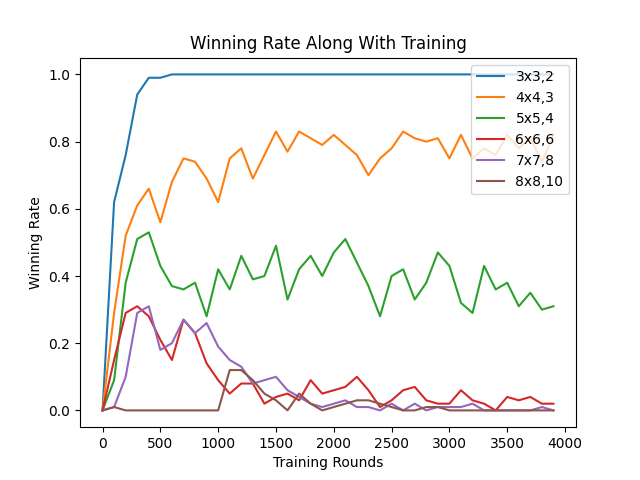
\includegraphics[height=6cm,width=6cm]{fig_1}
		\caption{winning rate along with training}  	
	\end{minipage}%  
	\hfill  
	\begin{minipage}[t]{0.5\linewidth}  	
		\centering  	
		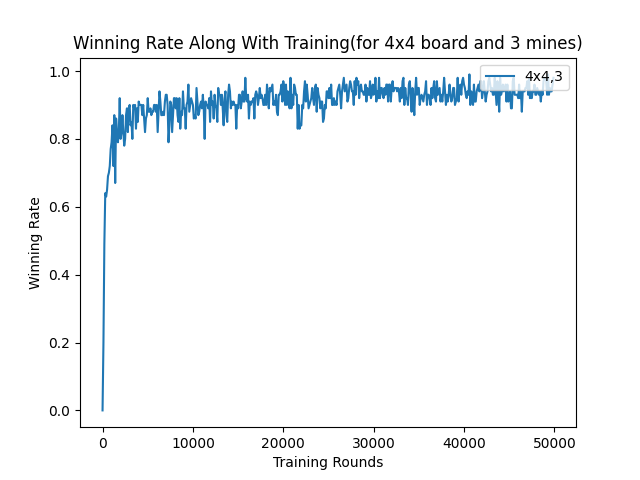
\includegraphics[height=6cm,width=6cm]{fig_2}  	
		\caption{winning rate along with traning(for $4\times4$ board and 3 mines}  	
	\end{minipage}
\end{figure}
\begin{table}
	\caption{average testing winning rates in 1000 rounds}
	\label{testing winning}
	\centering
	\begin{tabular}{cccc}
		\toprule
		Game model   & Average winning rate & Game model   & Average winning rate\\
		\midrule
		4x4 board, 3 mines & 84.29\%  & 6x6 board, 6 mines  &  4.29\%     \\
		5x5 board, 3 mines & 57.27\%  & 7x7 board, 8 mines  &  1.07\%    \\
		5x5 board, 4 mines & 26.50\%  & 8x8 board, 10 mines &  0.35\%    \\
		\bottomrule
	\end{tabular}
\end{table}

\section{Conculsions}
\label{headings}
In this project, some attemps were made to find a minesweeper solver with machine learning methods which could have a good winning rate with comparatively low complexity. With this belief, three algorithms are used. The first is a naive linear classifier. Due to its robust assumption, it holds a really low complexity but poor performance while training. Secondly, improving traditional Q-learning, Q-like-learning is developed. However, limited by laptop hardware, experiment on model with code cannot be conducted. Finally, we realize a back propagation neural network model and train it on $4\times4$ board. It shows good properties of convergence and acquires a relatively good winning rate around $90\%$. The model can be expanded to convolution neural network by masking the well-trained $4\times 4$ model on larger game sizes and achieve pretty good results.

Our models have great potential to hold much better performance. It can be improved by adjusting parameters to get a better network structure or applying an advanced convolutional neural network model. Also, we could try to implement the Q-like-learning algorithm in a better way on stronger hardwares to verify our theoretical analysis.




\section*{References}


\medskip

\small

[1] Luis, G\ \& Griffin, K\ (2015) Train a minesweeper solver. CS229.

[2] Kanye, R\ (2000) Minesweeper is NP-complete {\it The Mathematical Intelligencer, 22, 9-15.}

[3] Project webpage. {\it https://github.com/ryanbaldini/MineSweeperNeuralNet}

[4] Project webpage. {\it https://medium.com/@sakeshpusuluri123/activation-functions-and-weight-initialization-in-deep-learning-ebc326e62a5c}
\end{document}